\documentclass[12pt,a4paper]{article}
\usepackage[a4paper,top=1.5cm, bottom=1.5cm, left=1.5cm, right=1.5cm]{geometry}
\usepackage[T2A]{fontenc}
\usepackage[utf8]{inputenc}
\usepackage[russian]{babel}
\usepackage{amsmath}
\usepackage{amssymb}
\usepackage{hyperref}
\usepackage{graphicx}
\usepackage{floatrow}
\usepackage{booktabs}
\usepackage{wrapfig}
\usepackage{indentfirst}
\usepackage{lipsum}
\usepackage{subcaption}
\usepackage{float}
\usepackage{derivative}
\usepackage{enumitem}
\restylefloat{table}

\newcommand{\figref}[1]{(см. рис. \ref{#1})}
\newcommand{\e}[1]{\text{$\cdot10^{#1}$}}

\title{Лабораторная работа 3.4.1\\ Исследование диа- и парамагнетиков}
\author{Симанкович Александр \\ Б01-104}
\date{30.09.2022}

\begin{document}
	\maketitle
	
	\section*{Аннотация}
	
	В работе изучены свойства диамагнетика (Cu) и парамагнетика (Al). Измерены значения магнитной восприимчивости меди, алюминия, графита и вольфрама.
	
	\vspace{10pt}
	\noindent\textbf{Ключевые слова}: диамагнетики, парамагнетики.
	
	\section*{Введение}
		
	Применение парамагнетиков и диамагнетиков весьма ограничены. При это изучение свойств парамагнетиков и диамагнетиков дает экспериментальные результаты для построения теорий квантовой физики, физики кристаллов и других связанных областей, что в свою очередь имеет множество приложений.
	
	Данная работа была проведена в рамках учебного исследовательского курса в Московском физико-техническом институте. Целью работы ставится подтверждение теории, описывающей взаимодействия диа- и парамагнетиков с магнитным полем, а также определение их численных характеристик.
	
	\section*{Теоретическая модель}
	
	\subsection*{Диамагнетизм}
	
	Диамагнитный эффект характерен всем веществам. Данный эффект определяется микроскопическими 'токами', создающимися при помещении вещества в магнитное поле из-за эффекта электромагнитной индукции.
	
	\section*{Методика эксперимента}
	
	\subsection*{Оборудование и приборы}
	\begin{itemize}[itemsep = 0pt, parsep=0pt]
		\item электромагнит;
		\item аналитические весы;
		\item милливеберметр;
		\item регулируемый источник постоянного тока;
		\item образцы меди и алюминия;
	\end{itemize}
	
	\begin{wrapfigure}{r}{0.30\textwidth}
		\vspace{-80pt}
		\center{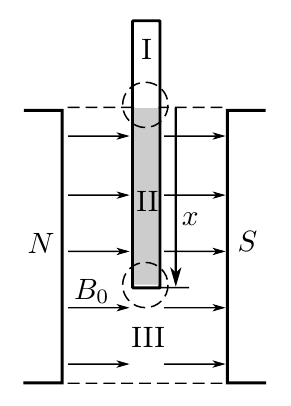
\includegraphics[width=\linewidth]{res/rod.png}}
		\caption{Схема взаимного расположения образца и магнита.}
		\label{img:rod}
	\end{wrapfigure}
	В данной работе для определения свойств образцов используется \textit{метод Гюи}. В нем в качестве образца выступает длинный тонкий стержень, один из концов которого помещается в зазор электромагнита \figref{img:rod}. 
	В зависимости от знака магнитной восприимчивости $\chi$ при включении электромагнита стержень будет втягиваться или выталкиваться из зазора.
	
	$$ F_M = \pdv{W_M}{x}_{B_0} \approx \chi \frac{B_0^2}{2 \mu_0} S. $$
	
	Таким образом, мы получили, что парамагнетики ($\chi > 0$) втягиваются в зазор электромагнита, а диамагнетики ($\chi < 0$) выталкиваются.
	
	\begin{figure}[h]
		\center{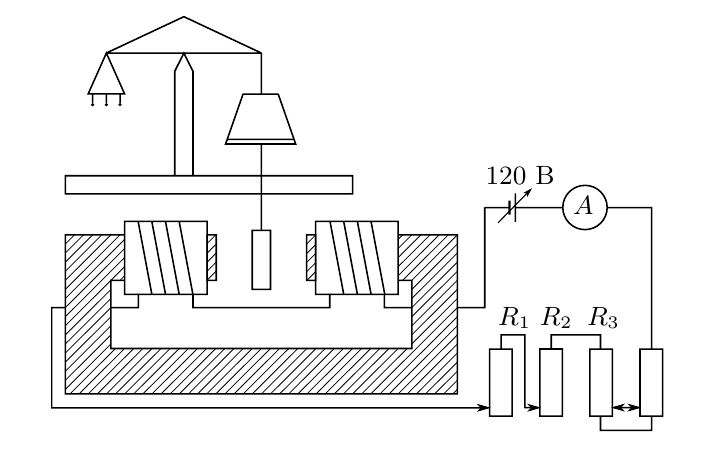
\includegraphics[width=0.6\linewidth]{res/scheme.png}}
		\caption{Схема установки.}
		\label{img:scheme}
	\end{figure}

	Схема установки представлена на рис. \ref{img:scheme}. В зазоре электромагнита с сердечником, питаемого от источника постоянного тока, создается магнитное поле. Поскольку размер зазора меньше размеров полюсов $l << \sqrt{S}$, то поле можно считать однородным.
	
	Для определения зависимости $B(I)$ проводится калибровка электромагнита с помощью веберметра.
	
	Для измерения магнитной восприимчивости будем находить силу, действующую на образец со стороны магнитного поля в электромагните. Для этого воспользуемся аналитическими весами. Изначальная масса образца измеряется при выключеном электромагните. После этого при включенном электромагните мы добиваемся равновесия весов. Перегрузка весов и будет являтся требуемой силой $\Delta P = F$.
	
	\section*{Результаты}
	
	\subsection*{Калибровка электромагнита}
	
	Проведем градуировку электромагнита. Для этого измерим зависимость $B(I)$, где $B$ -- модуль вектора индукции магнитного поле в зазоре, $I_M$ -- ток, протекающий через обмотки магнита. Измерения проведем милливеберметром M119 и миллитесламетром AKTAKOM ATE-8702. Погрешности данных приборов:
	$$ \varsigma_{\text{Вб}} = (0.015 \cdot \Phi + 0.05) \; \text{мВб} \quad \varepsilon_{\text{Тл}} = (0.05 \cdot B + 10) \; \text{мТл}$$
	Точность измерения $I_M$ определяется точностью амперметра $A_1$, встроенного в лабораторный блок питания GPR-11H30D: $$\varsigma_{A_1} = 0.005 \cdot I + 0.02 \; \text{А}$$
	
	Построим графики $B(I)$ по результатам измерения магнитного поля милливеберметром и миллитесламетром.
	
	\begin{figure}[H]
		\includegraphics[]{gen/electromagnet_BI.pdf}
		\caption{Зависимость поля в зазоре $B$ от протекающего тока $I$}
	\end{figure}
	
	Как видно из графика, калибровка обоими приборами совпадает в пределах погрешности. Для вычисления значения поля в последующих пунктах используется калибровка с помощью тесламетра.
	
	\subsection*{Измерение перегрузок}
	
	С помощью аналитических весов проведем измерения значения перегрузки $\Delta P$ при различных значениях поля $B$ в зазоре электромагнита. Измерения будем проводить как в прямом (\textit{рост}), так и в обратном (\textit{падение}) направлении.
	
	Первые измерения проводим для меди и алюминия. Построим графики:
	
	\begin{figure}[H]
		\includegraphics[]{gen/cu_al.pdf}
		\caption{Зависимость перегрузки $\Delta P$ от поля в зазоре $B$ для меди и алюминия}
	\end{figure}

	\begin{table}[h]
		\caption{Параметры графика $\Delta P(B^2)$ для меди}
		\input{gen/cu_mnk.tex}
	\end{table}
	
	\begin{table}[h]
		\caption{Параметры графика $\Delta P(B^2)$ для алюминия}
		\input{gen/al_mnk.tex}
	\end{table}
		
	На графиках наблюдаем линейную зависимость $\Delta P$ от $B^2$, как и ожидалось из теории.
	
	Рассчитаем значения магнитной восприимчивости $\chi$:
	
	$$\chi_{Cu} = -(1.08 \pm 0.03) \cdot 10^{-5} $$
	$$\chi_{Al} = +(2.17 \pm 0.03) \cdot 10^{-5} $$
	
	\begin{figure}[H]
		\includegraphics[]{gen/gr.pdf}
		\caption{Зависимость перегрузки $\Delta P$ от поля в зазоре $B$ для графита}
	\end{figure}
	
	\begin{table}[h]
		\caption{Параметры графика $\Delta P(B^2)$ для целого графита}
		\input{gen/gr_mnk.tex}
	\end{table}
	
	$$\chi_{Gr} = +(2.15 \pm 0.11) \cdot 10^{-4} $$
	
	\begin{figure}[H]
		\includegraphics[]{gen/wr_dbl.pdf}
		\caption{Зависимость перегрузки $\Delta P$ от поля в зазоре $B$ для вольфрама}
	\end{figure}
	
	\begin{table}[h]
		\caption{Параметры графика $\Delta P(B^2)$ для сдвоенного образца вольфрама}
		\input{gen/wr_dbl_mnk.tex}
	\end{table}
	
	$$\chi_{W} = +(7.24 \pm 0.26) \cdot 10^{-5} $$
	
	
	\section*{Заключение и выводы}
	
	
\end{document}